\section{HOODIE}
HOODIE ist eine JavaScript Bibliothek für offlinefähige Webapplikationen, die ein komplettes Backend zur Verfügung stellt.
Wird HOODIE für die Entwicklung einer Webanwendung verwendet, muss also lediglich das Frontend implementiert werden.
Den Rest erledigt die Bibliothek. Über eine integrierte Programmierschnittstelle kommuniziert die Anwendung mit dem von HOODIE zur Verfügung gestelltem Backend.
Über das \gls{API} können unter anderem BenutzerInnen authentifiziert, Daten gespeichert und synchronisiert werden~\cite{hoodie}.\\
Anhand der Abbildung \ref{fig:hoodie} wird erklärt wie HOODIE funktioniert.
%
\begin{figure}[H]
  \centering
  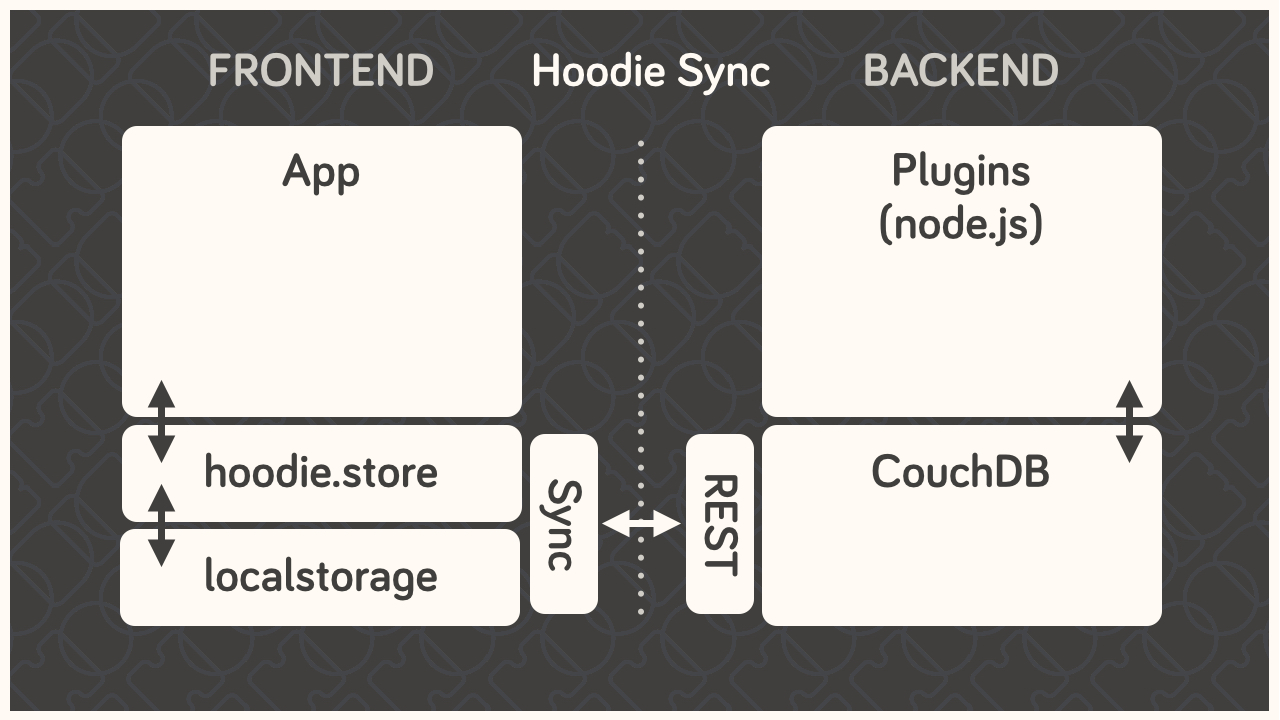
\includegraphics[width=0.8\textwidth]{hoodie}
  \grayRule
  \caption[HOODIE Architektur]{HOODIE Architektur~Quelle:~\cite{hoodie-how}}
  \label{fig:hoodie}
\end{figure}
%
Im Frontend--Bereicht ist die App zu sehen die über das HOODIE \gls{API} mit dem lokalen Speicher kommuniziert.
Die Anwendung spricht niemals direkt mit dem Server oder der Datenbank. Für die lokale Speicherung der Daten benutzt HOODIE intern PouchDB, was wiederum IndexedDB verwendet. Durch das lokale Speichern sind die Daten auch offline verfügbar. Dann werden über eine \gls{REST} Schnittstelle mit einer CouchDB synchronisiert.
In HOODIE haben alle AnwenderInnen ihre eigene private CouchDB.
Hinter der Datenbank befindet sich ein Server der auf die Daten in der CouchDB reagiert, die wiederum die Änderungen an den Client schickt ~\cite{hoodie-how}.
So können NutzerInnen nur auf ihre eigenen Daten zugreifen. Wenn es mehrere Geräte gibt, die mit einem Account assoziiert werden, werden die Änderungen von einem Gerät zuerst auf die serverseitige CouchDB synchronisiert, um dann von dort in die lokalen Datenbanken der anderen Geräte zu gelangen.\\
Dadurch, dass das Frontend und das Backend nicht direkt miteinander sprechen, ist die Funktionalität beider Komponenten auch dann gewährleistet, wenn die Verbindung zwischen ihnen unterbrochen wird~\cite{hoodie-how}.
% 
% CouchDB
% 
\sub{\label{chap:couch}CouchDB}
Apache CouchDB\tm ist ein \gls{DBMS} das seit 2005 als freie Software entwickelt wird. Die dokumentenorientierte Datenbank funktioniert sowohl als einzelne Instanz, als auch im Cluster. In einem Cluster kann ein Datenbanksserver auf einer beliebig großen Anzahl an Servern oder Virtuellen Maschinen ausgeführt werden.\\
% So kann die Datenschicht beliebig skaliert werden, um die Anforderungen vieler BenutzerInnen zu erfüllen.
CouchDB verwendet das \gls{HTTP}--Protokoll und \gls{JSON} als Datenformat, weswegen es in jeder webfähigen Anwendung leicht zu integrieren ist. CouchDB wird über ein \gls{REST}ful \gls{HTTP} \gls{API} angesprochen. So können Daten über die für den \gls{REST}ful Services standardisierten Methoden wie zum Beispiel GET, POST, PUT, DELETE abgerufen oder manipuliert werden.\\\\
%
%
Das implementierte Replikationsmodell erlaubt die Synchronisation bzw. bidirektionale Replikation zu verschiedenen Geräten, was das besondere Merkmal von CouchDB ist.
Die genaue Funktionsweise des Protokolls ist in \autoref{chap:replication} detailliert beschrieben.\\
% 
Dank des Replikations--\gls{API} kann kann sich eine CouchDB kontinuierlich und eigenständig mit einer anderen Datenbank die dasselbe Protokoll implementiert, synchronisieren.
Wenn Konflikte auftreten, beispielsweise durch gleichzeitiges Bearbeiten eines Dokuments von zwei Personen ohne Netzwerkverbindung, werden diese als solche markiert, jedoch nicht von selbst aufgelöst~\cite{couch}. Die Lösung der Konflikte muss in der Anwendung implementiert sein.
So kann gewährleistet werden, dass keinerlei Daten verloren gehen.\\\\
%
%
CouchDB ist für Server konzipiert. Für Browser gibt es \hyperref[chap:pouch]{PouchDB} und für native iOS- und Android--\glspl{App} wurde Couchbase Lite entwickelt.
Des Weiteren gibt es noch die Datenbanken Couchbase und Cloudant.
Alle verwenden das CouchDB \hyperref[chap:replication]{Replikationsprotokoll} und können Daten miteinander replizieren und~\cite{couch}.
%
% Pouch
%
\sub{\label{chap:pouch}PouchDB}
% Als Ergänzung zu CouchDB kann PouchDB verwendet werden.
PouchDB ist die Java"-Script Implementierung von CouchDB.
Sie ist quelloffen und wurde so konzipiert, dass sie in allen modernen Browsers läuft. Dort ermöglicht PouchDB es Daten zu persistieren, sodass sowohl offline als auch online verfügbar sind.
PouchDB speichert die Daten in IndexedDB und stellt für das Abrufen und Manipulieren derer ein einheitliches \gls{API} zur Verfügung.\\
Sind die Daten einmal offline gespeichert können sie, dank des CouchDB \hyperref[chap:replication]{Replikationsprotokolls}, sobald die Awendung wieder online ist mit CouchDB kompatiblen Servern synchronisiert werden~\cite{pouch}.